%% Преамбула TeX-файла

% 1. Стиль и язык
\documentclass[utf8x,times, 14pt]{G7-32} % Стиль (по умолчанию будет 14pt)

% Остальные стандартные настройки убраны в preamble.inc.tex.
\sloppy

% Настройки стиля ГОСТ 7-32
% Для начала определяем, хотим мы или нет, чтобы рисунки и таблицы нумеровались в пределах раздела, или нам нужна сквозная нумерация.
\EqInChapter % формулы будут нумероваться в пределах раздела
\TableInChapter % таблицы будут нумероваться в пределах раздела
\PicInChapter % рисунки будут нумероваться в пределах раздела

% Добавляем гипертекстовое оглавление в PDF
\usepackage[
bookmarks=true, colorlinks=true, unicode=true,
urlcolor=black,linkcolor=black, anchorcolor=black,
citecolor=black, menucolor=black, filecolor=black,
]{hyperref}

\AfterHyperrefFix

\usepackage{microtype}% полезный пакет для микротипографии, увы под xelatex мало чего умеет, но под pdflatex хорошо улучшает читаемость

% Тире могут быть невидимы в Adobe Reader
\ifInvisibleDashes
\MakeDashesBold
\fi

\usepackage{graphicx}   % Пакет для включения рисунков

% С такими оно полями оно работает по-умолчанию:
% \RequirePackage[left=20mm,right=10mm,top=20mm,bottom=20mm,headsep=0pt,includefoot]{geometry}
% Если вас тошнит от поля в 10мм --- увеличивайте до 20-ти, ну и про переплёт не забывайте:
\geometry{right=20mm}
\geometry{left=30mm}
\geometry{bottom=20mm}
\geometry{ignorefoot}% считать от нижней границы текста


% Пакет Tikz
\usepackage{tikz}
\usetikzlibrary{arrows,positioning,shadows}

% Произвольная нумерация списков.
\usepackage{enumerate}

% ячейки в несколько строчек
\usepackage{multirow}

% itemize внутри tabular
\usepackage{paralist,array}

%\setlength{\parskip}{1ex plus0.5ex minus0.5ex} % разрыв между абзацами
\setlength{\parskip}{1ex} % разрыв между абзацами
\usepackage{blindtext}

% Центрирование подписей к плавающим окружениям
%\usepackage[justification=centering]{caption}

\usepackage{newfloat}
\DeclareFloatingEnvironment[
placement={!ht},
name=Equation
]{eqndescNoIndent}
\edef\fixEqndesc{\noexpand\setlength{\noexpand\parindent}{\the\parindent}\noexpand\setlength{\noexpand\parskip}{\the\parskip}}
\newenvironment{eqndesc}[1][!ht]{%
    \begin{eqndescNoIndent}[#1]%
\fixEqndesc%
}
{\end{eqndescNoIndent}}


\usepackage{pgfplots}
\pgfplotsset{width=\linewidth,compat=1.9}


% Настройки листингов.
\ifPDFTeX
% 8 Листинги

\usepackage{listings}
% \usepackage{listingsutf8}

% Значения по умолчанию
\lstset{
  basicstyle= \scriptsize,
  breakatwhitespace=true,% разрыв строк только на whitespacce
  breaklines=true,       % переносить длинные строки
%   captionpos=b,          % подписи снизу -- вроде не надо
  inputencoding=koi8-r,
  numbers=left,          % нумерация слева
  numberstyle=\footnotesize,
  showspaces=false,      % показывать пробелы подчеркиваниями -- идиотизм 70-х годов
  showstringspaces=false,
  showtabs=false,        % и табы тоже
  stepnumber=1,
  tabsize=4,              % кому нужны табы по 8 символов?
  frame=single
}

% Стиль для псевдокода: строчки обычно короткие, поэтому размер шрифта побольше
\lstdefinestyle{pseudocode}{
  basicstyle=\small,
  keywordstyle=\color{black}\bfseries\underbar,
  language=Pseudocode,
  numberstyle=\footnotesize,
  commentstyle=\footnotesize\it
}

% Стиль для обычного кода: маленький шрифт
\lstdefinestyle{realcode}{
  basicstyle=\scriptsize,
  numberstyle=\footnotesize
}

% Стиль для коротких кусков обычного кода: средний шрифт
\lstdefinestyle{simplecode}{
  basicstyle=\footnotesize,
  numberstyle=\footnotesize
}

% Стиль для BNF
\lstdefinestyle{grammar}{
  basicstyle=\footnotesize,
  numberstyle=\footnotesize,
  stringstyle=\bfseries\ttfamily,
  language=BNF
}

% Определим свой язык для написания псевдокодов на основе Python
\lstdefinelanguage[]{Pseudocode}[]{Python}{
  morekeywords={each,empty,wait,do},% ключевые слова добавлять сюда
  morecomment=[s]{\{}{\}},% комменты {а-ля Pascal} смотрятся нагляднее
  literate=% а сюда добавлять операторы, которые хотите отображать как мат. символы
    {->}{\ensuremath{$\rightarrow$}~}2%
    {<-}{\ensuremath{$\leftarrow$}~}2%
    {:=}{\ensuremath{$\leftarrow$}~}2%
    {<--}{\ensuremath{$\Longleftarrow$}~}2%
}[keywords,comments]

% Свой язык для задания грамматик в BNF
\lstdefinelanguage[]{BNF}[]{}{
  morekeywords={},
  morecomment=[s]{@}{@},
  morestring=[b]",%
  literate=%
    {->}{\ensuremath{$\rightarrow$}~}2%
    {*}{\ensuremath{$^*$}~}2%
    {+}{\ensuremath{$^+$}~}2%
    {|}{\ensuremath{$|$}~}2%
}[keywords,comments,strings]

\lstdefinelanguage[]{MyPs}[]{}{
  morekeywords={each,empty,wait,do},% ключевые слова добавлять сюда
  morecomment=[s]{\{}{\}},
  literate=
    {\\\\}{\ensuremath{$\vartriangleright$}~}2%
    {->}{\ensuremath{$\rightarrow$}~}2%
    {<-}{\ensuremath{$\leftarrow$}~}2%
    {==}{\ensuremath{$=$}~}2%
    {!=}{\ensuremath{$\neq$}~}2%
    {:=}{\ensuremath{$\leftarrow$}~}2%
    {\\in}{\ensuremath{$ \in $}~}2%
    {<--}{\ensuremath{$\Longleftarrow$}~}2%
    {\\times}{\ensuremath{$\times$}~}2%
    {<=}{\ensuremath{$\leq$}~}2%
    {>=}{\ensuremath{$\geq$}~}2%
}[keywords,comments,strings]

% Подписи к листингам на русском языке.
\renewcommand\lstlistingname{Листинг}
\renewcommand\lstlistlistingname{Листинги}



\else
\usepackage{local-minted}
\fi

\usepackage{indentfirst}
\usepackage{ulem} % Нормальное нижнее подчеркивание

% Дополнительное окружения для подписей
\usepackage{array}
\newenvironment{signstabular}[1][1]{
	\renewcommand*{\arraystretch}{#1}
	\tabular
}{
	\endtabular
}


\newcommand{\frc}[2]{\raisebox{2pt}{$#1$}\big/\raisebox{-3pt}{$#2$}}    % a/b, a выше, b ниже

\renewcommand{\labelenumi}{\arabic{enumi})}
\renewcommand{\labelenumii}{\asbuk{enumii})}

% Полезные макросы листингов.
% Любимые команды
\newcommand{\Code}[1]{\textbf{#1}}

\newenvironment{signstabular}[1][1]{
	\renewcommand*{\arraystretch}{#1}
	\tabular
}{
	\endtabular
}



\newcommand{\frc}[2]{\raisebox{2pt}{$#1$}\big/\raisebox{-3pt}{$#2$}}    % a/b, a выше, b ниже

\renewcommand{\labelenumi}{\arabic{enumi})}
\renewcommand{\labelenumii}{\asbuk{enumii})}



\usepackage[T2A]{fontenc} % Поддержка русских букв
% \usepackage[utf8]{inputenc} % Кодировка utf8
% \usepackage[english, russian]{babel} % Языки: русский, английский
% \usepackage{pscyr} % Нормальные шрифты

\usepackage{algorithm}
\usepackage{algpseudocode}
\floatname{algorithm}{Псевдокод}

\algrenewcommand\algorithmicwhile{\textbf{До тех пока}}
\algrenewcommand\algorithmicdo{\textbf{выполнить}}
\algrenewcommand\algorithmicrepeat{\textbf{Повторять}}
\algrenewcommand\algorithmicuntil{\textbf{Пока выполняется}}
\algrenewcommand\algorithmicend{\textbf{Конец}}
\algrenewcommand\algorithmicif{\textbf{Если}}
\algrenewcommand\algorithmicelse{\textbf{иначе}}
\algrenewcommand\algorithmicthen{\textbf{тогда}}
\algrenewcommand\algorithmicfor{\textbf{Цикл}}
\algrenewcommand\algorithmicforall{\textbf{Для всех}}
\algrenewcommand\algorithmicfunction{\textbf{Функция}}
\algrenewcommand\algorithmicprocedure{\textbf{Процедура}}
\algrenewcommand\algorithmicloop{\textbf{Зациклить}}
\algrenewcommand\algorithmicrequire{\textbf{Условия:}}
\algrenewcommand\algorithmicensure{\textbf{Обеспечивающие условия:}}
\algrenewcommand\algorithmicreturn{\textbf{Возвратить}}
\algrenewtext{EndWhile}{\textbf{Конец цикла}}
\algrenewtext{EndLoop}{\textbf{Конец зацикливания}}
\algrenewtext{EndFor}{\textbf{Конец цикла}}
\algrenewtext{EndFunction}{\textbf{Конец функции}}
\algrenewtext{EndProcedure}{\textbf{Конец процедуры}}
\algrenewtext{EndIf}{\textbf{Конец условия}}
\algrenewtext{EndFor}{\textbf{Конец цикла}}
\algrenewtext{BeginAlgorithm}{\textbf{Начало алгоритма}}
\algrenewtext{EndAlgorithm}{\textbf{Конец алгоритма}}
\algrenewtext{BeginBlock}{\textbf{Начало блока. }}
\algrenewtext{EndBlock}{\textbf{Конец блока}}
\algrenewtext{ElsIf}{\textbf{иначе если }}

\renewcommand{\thealgorithm}{\thechapter.\arabic{algorithm}}%

\makeatletter
\@addtoreset{algorithm}{chapter}% algorithm counter resets every chapter
\makeatother



% Fix breaking algos per page 
\makeatletter
\newenvironment{breakablealgorithm}
  {% \begin{breakablealgorithm}
   \begin{center}
     \refstepcounter{algorithm}% New algorithm
     \hrule height.8pt depth0pt \kern2pt% \@fs@pre for \@fs@ruled
     \renewcommand{\caption}[2][\relax]{% Make a new \caption
       {\raggedright\textbf{\fname@algorithm~\thealgorithm} ##2\par}%
       \ifx\relax##1\relax % #1 is \relax
         \addcontentsline{loa}{algorithm}{\protect\numberline{\thealgorithm}##2}%
       \else % #1 is not \relax
         \addcontentsline{loa}{algorithm}{\protect\numberline{\thealgorithm}##1}%
       \fi
       \kern2pt\hrule\kern2pt
     }
  }{% \end{breakablealgorithm}
     \kern2pt\hrule\relax% \@fs@post for \@fs@ruled
   \end{center}
  }
\makeatother



\begin{document}

\frontmatter % выключает нумерацию ВСЕГО; здесь начинаются ненумерованные главы: реферат, введение, глоссарий, сокращения и прочее.

\begin{titlepage}
    \thispagestyle{empty}

    \noindent\begin{minipage}{0.05\textwidth}
        
\includegraphics[scale=0.3]{img/bmstu.png}
    \end{minipage}
    \hfill
    \begin{minipage}{0.85\textwidth}\raggedleft
        \begin{center}
            \fontsize{12pt}{0.3\baselineskip}\selectfont \textbf{Министерство науки и высшего образования Российской Федерации \\ Федеральное государственное бюджетное образовательное учреждение \\ высшего образования \\ <<Московский государственный технический университет \\ имени Н.Э. Баумана \\ (национальный исследовательский университет)>> \\ (МГТУ им. Н.Э. Баумана)}
        \end{center}
    \end{minipage}

    \begin{center}
        \fontsize{12pt}{0.1\baselineskip}\selectfont
        \noindent\makebox[\linewidth]{\rule{\textwidth}{4pt}} \makebox[\linewidth]{\rule{\textwidth}{1pt}}
    \end{center}

    \begin{flushleft}
        \fontsize{12pt}{0.8\baselineskip}\selectfont

        ФАКУЛЬТЕТ \uline{
            Информатика и системы управления
            \hfill}

        КАФЕДРА \uline{\mbox{\hspace{4mm}}
            Программное обеспечение ЭВМ и информационные технологии
            \hfill}
    \end{flushleft}

    \vfill

    \begin{center}
        \fontsize{20pt}{\baselineskip}\selectfont

        \textbf{РАСЧЕТНО-ПОЯСНИТЕЛЬНАЯ ЗАПИСКА}

        \textbf{\textit{К КУРСОВОЙ РАБОТЕ}}

        \textbf{\textit{НА ТЕМУ:}}
    \end{center}

    \begin{center}
        \fontsize{18pt}{0.6cm}\selectfont

        Разработка   программного   обеспечения   для генерации размытия движения полигональных моделей

    \end{center}

    \vfill

    \begin{table}[h!]
        \fontsize{12pt}{0.7\baselineskip}\selectfont
        \centering
        \begin{signstabular}[0.7]{p{7.25cm} >{\centering\arraybackslash}p{4cm} >{\centering\arraybackslash}p{4cm}}
            Студент группы ИУ7-54Б & \uline{\mbox{\hspace*{4cm}}} & \uline{\hfill В.Н. Ларин  \hfill} \\
            & \scriptsize (Подпись, дата) & \scriptsize (И.О. Фамилия)
        \end{signstabular}

        \vspace{\baselineskip}

        \begin{signstabular}[0.7]{p{7.25cm} >{\centering\arraybackslash}p{4cm} >{\centering\arraybackslash}p{4cm}}
            Руководитель курсовой работы & \uline{\mbox{\hspace*{4cm}}} & \uline{\hfill А.А. Волкова \hfill} \\
            & \scriptsize (Подпись, дата) & \scriptsize (И.О. Фамилия)
        \end{signstabular}

        \vspace{\baselineskip}

        \begin{signstabular}[0.7]{p{7.25cm} >{\centering\arraybackslash}p{4cm} >{\centering\arraybackslash}p{4cm}}
            Консультант & \uline{\mbox{\hspace*{4cm}}} & \uline{\hfill  \hfill} \\
            & \scriptsize (Подпись, дата) & \scriptsize (И.О. Фамилия)
        \end{signstabular}
    \end{table}

    \vfill

    \begin{center}
        \normalsize \textit{\textbf{2021} г.}
    \end{center}
\end{titlepage}



% \begin{executors}
% \personalSignature{Первый исполнитель}{ФИО}

% \personalSignature{Второй исполнитель}{ФИО}
% \end{executors}


%\listoffigures                         % Список рисунков

%\listoftables                          % Список таблиц

%\NormRefs % Нормативные ссылки 
% Команды \breakingbeforechapters и \nonbreakingbeforechapters
% управляют разрывом страницы перед главами.
% По-умолчанию страница разрывается.

% \nobreakingbeforechapters
% \breakingbeforechapters

% Также можно использовать \Referat, как в оригинале
\begin{abstract}

    Отчет содержит \pageref{LastPage}\,стр.%
    \ifnum \totfig >0
    , \totfig~рис.%
    \fi
    \ifnum \tottab >0
    , \tottab~табл.%
    \fi
    %
    \ifnum \totbib >0
    , \totbib~источн.%
    \fi
    %
    \ifnum \totapp >0
    , \totapp~прил.%
    \else
    .%
    \fi


    % Это пример каркаса расчётно-пояснительной записки, желательный к использованию в РПЗ проекта по курсу РСОИ
    \nocite{*}.

    % Данный опус, как и более новые версии этого документа, можно взять по адресу (\url{https://github.com/latex-g7-32/latex-g7-32}).

    % Текст в документе носит совершенно абстрактный характер.

\end{abstract}

%%% Local Variables: 
%%% mode: latex
%%% TeX-master: "rpz"
%%% End: 


\tableofcontents

\printnomenclature % Автоматический список сокращений

\Introduction
Синтез реалистичных изображений в настоящее время переживает смену парадигмы в сторону производства контента в реальном времени. Современные игровые движки способны в режиме реального времени воспроизводить многие реалистичные графические приемы, которые традиционно требовали большого количества времени на вычисления \cite{RONNOW202136}.  
\par
Игровым сценам присущи движения тех или иных объектов, например, бег игрока, полет самолетов и другие. В отличие от снимков движущихся объектов, сделанных фотокамерой, отрисованное изображение будет четким, что лишает зрителя информации о движении объекта. Из-за этого отрисованная анимация объектов может казаться разорванной \cite{Navarro11}.   Данная проблема актуальна, так как рынок видеоигр стремительно развивается, а вычислительной мощности устройств не всегда хватает, чтобы достичь достаточной частоты обновления экрана.
\par
Данную проблему можно решить с помощью добавления на сгенерированное изображение размытия движения. Размытие движения - это эффект, проявляющийся в виде видимых полос, возникающих при движении объекта перед записывающим устройством. Размытие может быть вызвано движением объекта и/или камеры.  Размытие может наблюдаться как на неподвижных фотографиях, так и в последовательностях изображений \cite{Navarro11}.  

% Синтез реалистичных изображений в настоящее время переживает смену парадигмы в сторону производства контента в реальном времени. Современные игровые движки способны в режиме реального времени воспроизводить многие реалистичные графические приемы, которые традиционно требовали большого количества времени на вычисления.
% \par
% Некоторые из этих приемов все еще грубо аппроксимируются, что приводит к появлению видимых артефактов. Для достижения эффекта интерактивности и скрытию этих артифактов можно использовать размытие. Одним из таких эффектов является размытие движения, которое необходимо для представления движущихся объектов. Размытие движения - это распространенный оптический эффект на фотографиях и видео, который возникает, когда положение объектов меняется относительно точки зрения камеры в течение промежутка времени, когда затвор камеры открыт. Если объекты движутся быстро, или интервал между затворами достаточно длинный, то объекты оставляют размытые полосы в направлении движения. Важно воспроизвести этот эффект для синтеза захватывающих и более правдоподобных сцен, имитации определенных моделей камер или достижения художественных эффектов.
% \par
% Размытие движения - это эффект, проявляющийся в виде видимых полос, возникающих при движении
% объекта перед записывающим устройством. Это результат сочетания видимого движения в сцене и
% особенностей средства формирования изображения, которое объединяет свет в течение ограниченного времени съемки.
% \par
% Это относительное движение может быть вызвано движением объекта и движением камеры
% и может наблюдаться как на неподвижных фотографиях, так и в последовательностях изображений.
% В целом, последовательности, содержащие умеренное размытие движения, воспринимаются как
% естественные, в то время как его полное отсутствие приводит к рывкам и потере реалистичности.
% \par
% Размытие движения для синтезированных изображений является активной областью исследований
% с начала 1980-х годов. В отличие от записанных видеоматериалов, которые автоматически
% размывают движения, алгоритмы рендеринга должны явно моделировать его.
% \par
% В данной работе описывается происхождение этого явления и подробно рассматриваются алгоритмические решения, которые были найдены для его моделирования.
% \par
Целью работы является разработка ПО для генерации эффекта размытия движения полигональных моделей. Для достижения поставленной цели необходимо решить следующие задачи:

\begin{itemize}
    \item определить требования для генерации смаза движения;
    \item проанализировать существующие методы генерации смаза движения;
    \item проанализировать существующие методы генерации объемного изображения;
    \item реализовать генерацию объемного изображения с эффектом размытия движения полигональных моделей;
    \item провести сравнение временных и визуальных характеристик алгоритмов генерации смаза.
\end{itemize}



% Проверяем как у нас работают сокращения, обозначения и определения "---
% MAX,
% \Abbrev{MAX}{Maximus ""--- максимальное значение параметра}
% API
% \Abbrev{API}{application programming interface ""--- внешний интерфейс взаимодействия с приложением}
% с обратным прокси.
% \Define{Обратный прокси}{тип прокси-сервера, который ретранслирует}





\mainmatter % это включает нумерацию глав и секций в документе ниже

\chapter{Аналитический раздел}
\label{cha:analysis}
В данном разделе приведены основные сведения о размытие движения, о методах и алгоритмах его программной генерации.

\section{Природа размытия движения}

\subsection{Причины появления смаза}

Причины возникновения размытия изображений при съёмке камерой связаны со способом захвата изображения. Свет попадает на светочувствительную матрицу устройства. Затвор и диафрагма влияют на количество света, попавшего на матрицу. Затвор ограничивает время, в течение которого свет попадает на матрицу и формируется итоговое изображение. Данное время называется выдержкой.
\par
После открытия затвора матрица начинает аккумулировать весь свет, попавший на неё. Так как во время движения объекта отраженные лучи света меняют своё положения, то во время выдержки все проекции объекта на плоскость матрицы будут запечатлены на итоговом изображении.
\par
Данный процесс выдержки может быть формализован с помощью уравнения \eqref{F:F2_1_1} . Во время съемки сцены,  представляет собой содержимое плоскости изображения. Захваченный свет является результатом аккумулирования входящего излучения $L$ в течение времени выдержки $\Delta T$. Функция $f$ моделирует влияние оптики, затвора, диафрагмы, светочувствительности матрицы.
\par
\begin{eqndesc}
    \begin{equation}
        I = \int_{\Delta T} f(t) \cdot L(t) dt
        \label{F:F2_1_1}
    \end{equation}
    , где 
    $I$ "--- выходная интенсивность изображения;\\        
    $\Delta T$ "--- время выдержки;\\        
    $L(t)$ "--- входящее излучение на матрицы;\\        
    $f(t)$ "--- влияние оптики, затвора и прочих физических характеристик захвата излучения.        
\end{eqndesc}
\par
Уравнение \eqref{F:F2_1_1} дает представления о характеристиках получаемых изображений  \cite{Navarro11}. Можно сказать, что финальное изображения состоит из объединения моментальных снимков. Моментальный снимок - это снимок с временем выдержки, стремящемся к нулю.

\subsection{Описание характеристик смаза}
\label{cha:analysis_charestic}
Для изображения кадра перемещения сферы радиуса, соизмеримого с одним пикселем, необходимо отобразить путь пройденный этой сферой за время выдержки $\Delta T$. Так как любой объект можно представить в виде набора точек, то конечное изображение будет иметь вид следа перемещения объекта за время выдержки.
\par
Для упрощения задачи характеристики смаза, кривую перемещения любого тела можно представить в виде ломанной линии, где каждая точка ломанной есть точка времени начала/окончания выдержки. Такое упрощение возможно, так как время выдержки обычно равно периоду обновления экрана (При частоте обновления кадра 25 Гц выдержка равна 40 мс). Тогда любой путь объекта во время выдержки будет его перемещением. Для единичного пикселя смаз будет представлять собой отрезок, соединяющий точки нахождения пикселя в моменты времени начала и окончания выдержки.
\par
Из выше указанных замечаний можно выдвинуть следующие требования для генерации смазывания движущихся объектов:
\begin{enumerate}
    \item Смаз содержит изображения объекта в моменты времени начала и окончания выдержки;
    \item Смазывание формируется вдоль вектора движения объекта;
    \item Продолжительность смаза зависит от скорости движения объекта;
    \item Объекты без движения не подвергаются смазыванию;
    \item Смаз не терпит разрывов;
    \item Интенсивность изображения без движения соизмерима с интенсивностью смазанного изображения.
\end{enumerate}

\section{Методы размытия движения}

\subsection{Размытие движения с помощью накопительного буфера}
\label{cha:analysis_acum}

Одним из первых решений, которое было предложено - это склеивание нескольких отрендеренных изображений   \cite{Haeberli90}. Заметим, что интенсивность изображения должна быть соизмерима с начальной. С учетом данного утверждения получим формулу \eqref{F:F202}.
\begin{eqndesc}
    \begin{equation}\label{F:F202}
        I(t, \Delta T, N) = \frac{ \sum_{i=0}^{N} { V({t - \frac{i}{N} \cdot \Delta T})}}{N}
    \end{equation}
    \\
    где $t$ "--- время окончания выдержки \\
    $\Delta T$ "--- продолжительность выдержки \\
    $V(t)$ "--- мгновенный снимок в момент времени $t$\\
    $N$ "--- количество мгновенных снимков \\
    $I(t, \Delta T, N)$ "--- изображение с выдержкой $\Delta T$
\end{eqndesc}

Для достижения наивысшей скорости отрисовки изображения при генерации видео ряда необходимо накапливать результаты генерации последних $N$ моментальных снимков в буфере. Постоянность выдержки $\Delta T$ и частоты обновления экрана $fps$  позволяет на каждой итерации отрисовать следующее количество новых кадров  $k = \frac{N}{fps \cdot \Delta T}$, $k \in Z$
\par
Очевидно, что достигается максимальная скорость работы алгоритма при $k = 1$, т.е. когда $fps = \frac{N}{\Delta T}$


\begin{table}[ht]
    \caption{Зависимость частоты кадров от количества мгновенных снимков и времени выдержки}
    \begin{tabular}{|c|r|r|r|r|}
        \hline
        $\Delta T$, c & $N = 8$ & $N=16$ & $N=32$ & $N=64$ \\
        \hline
        $1$           & 8      & 16    & 32    & 64    \\
        $\frc{1}{2}$  & 16     & 32    & 64    & 128   \\
        $\frc{1}{4}$  & 32     & 64    & 128   & 256   \\
        $\frc{1}{8}$  & 64     & 128   & 256   & 512   \\
        $\frc{1}{16}$ & 128    & 256   & 512   & 1024  \\
        \hline
    \end{tabular}
    \label{tab:acum_table}
\end{table}

Проанализировав зависимость частоты кадров от количества мгновенных снимков и времени выдержки (таблица \ref{tab:acum_table}), можно прийти к следующему выводу. Чтобы получить изображение с малой выдержкой при большом количестве семплов нужно иметь большую частоту генерации кадров, что становится преградой для реализации размытия в режиме реального времени данным методом.

\subsection{Размытие движения с помощью скорости пикселя}
\label{cha:analysis_pixelblur}


В пункте \ref{cha:analysis_charestic} были сделаны предположения о природе смаза. Если рассматривать каждый пиксель изображения за время выдержки, то можно восстановить путь пройденный каждым пикселем с помощью мгновенной скорости каждого пикселя в момент начала/окончания выдержки.


\par
Для реализации такого размытия можно использовать следующую идею. Цвет каждого пикселя размытого изображения представить, как среднее арифметическое цветов пикселей вдоль вектора направления скорости вычисляемого пикселя   \cite{GpuGems2008}. Данная идея представлена в формуле \eqref{F:F2_2_1}. 

\begin{eqndesc}
    \begin{equation}\label{F:F2_2_1}
        I(x,y) = \frac{\sum_{i=0}^{N} {V(x + i \cdot v_x, y + i \cdot v_y)}}{N}
    \end{equation}
    \\
    где $x,y$ "--- координаты пикселя \\
    $v$ "--- мгновенная скорость размываемого пикселя  \\
    $V(x,y)$ "--- цвет пикселя мгновенного снимка \\
    $I(x,y)$ "--- цвет размытого пикселя
\end{eqndesc}



Данный подход позволяет генерировать размытие по одному снимку. Данный способ намного быстрее предыдущего, но обладает не идеальными графическими параметрами (рисунок \ref{fig:pixel_blur}).


\begin{figure}[h]
    \centering
    \begin{minipage}[h]{0.49\linewidth}
        \center{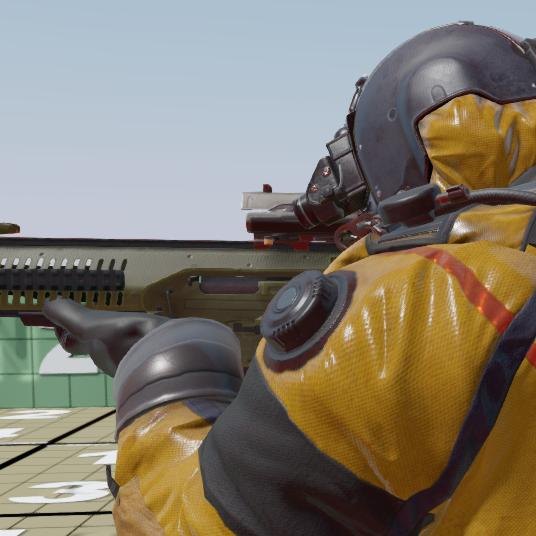
\includegraphics[width=0.5\linewidth]{img/blur_1.jpg} \\ а)}
    \end{minipage}
    \hfill
    \begin{minipage}[h]{0.49\linewidth}
        \center{
\includegraphics[width=0.5\linewidth]{img/blur_2.jpg} \\ б)}
    \end{minipage}
    \caption{Сравнение смаза. \\ а) Исходное изображение б) Изображение с размытием по скорости пикселя}
    \label{fig:pixel_blur}
\end{figure} 

\par
Данный метод оставляет резкую границу раздела заднего плана и смазываемого изображения. Это происходит из-за резкого перепада скорости фона и движущегося тела. Также при перекрытии движущегося тела статическим образуются артефакты отрисовки на границе тел. Неподвижное тело не смазывается, но на границе тел скорость резко меняет свое значение, и в соответствии с формулой \eqref{F:F2_2_1} интенсивность пикселя будет составляться и из части изображения неподвижного тела.
\par
Из выше сказанных слов делаем вывод, что данный метод смазывания работает без видимых артефактов  при равномерно-распределенной скорости каждого пикселя, например, при смене ракурса камеры.

\subsection{Размытие движения с помощью максимальной скорости движения участка изображения и буфера глубины}
\label{cha:analysis_mcgiure}

Проблему резких границ размытия было предложено решать с помощью снижения размерности буфера скоростей и анализа соседних участков буфера. Изображение разбивается на участки размера $k \times k$ пикселей, и для каждого участка ищется максимальная скорость. Такое преобразование из буфера скоростей пикселей можно сделать по формуле \eqref{F:F2_3_1}.
\begin{eqndesc}
    \begin{equation}\label{F:F2_3_1}
        TileMax[x,y] = \max_{u \in [o ; k)} {
        \max_{v \in [o ; k)} {v [kx + u; ky + v]}
        }
    \end{equation}
    , где $\max$ "--- максимальный вектор по длине; \\
    $v$ "---  буфер скоростей;\\
    $k$ "---  размерность участка.

\end{eqndesc}

Чтобы проанализировать все пиксели, которые вносят вклад в размытие того или иного пикселя необходимо, чтобы $|v[x,y]| \le k $ \space $\forall x,y $. Следующим шагом предлагается найти доминирующую скорость для соседей участка и самого участка.


Использование буфера максимальной скорости движения участков, задаваемого уравнение \eqref{F:F2_3_2}, решает проблему резких границ размытия.

\begin{eqndesc}
    \begin{equation}\label{F:F2_3_2}
        NeighborMax[x,y] = \max_{u \in [-1 ; 1]} {
            \max_{v \in [-1 ;1]} {TileMax [x + u; y + v]}
        }
    \end{equation}
    , где $\max$ "--- максимальный вектор по длине; \\
    $TileMax$ "---  буфер максимальных скоростей участков по формуле \eqref{F:F2_3_1}.
\end{eqndesc}

В методе размытия с помощью скорости пикселя суммировался цвет всех пикселей, даже тех, которые не являлись частью смаза текущего объекта. Чтобы решить данную проблему, было предложено при расчете каждого пикселя $A$ анализировать вклад $\alpha_i$ для каждого соседнего пикселя $B_i$ вдоль  вектора скорости $NeighborMax[\frac{A_x}{k}, \frac{A_y}{k}]$. Морган Макгуайр предложил считать, что пиксель $B_i$ вносит вклад $\alpha_i$ в смаз пикселя $A$ при следующих условиях:
\begin{enumerate}
    \item Условия вклада переднего плана
          \begin{enumerate}
              \item пиксель $B_i$ ближе к наблюдателю чем $A$
              \item пиксель $A$ находится в пределах разброса точек $B_i$;
          \end{enumerate}
    \item Условия вклада фона
          \begin{enumerate}
              \item пиксель $B_i$ дальше от наблюдателя чем $A$
              \item $B_i$ находится в пределах разброса точек $A$
          \end{enumerate}
    \item Условие для единого тела
          \begin{enumerate}
              \item пиксели $A$ и $B_i$ находятся в пределах разброса точек друг друга;
          \end{enumerate}
\end{enumerate}


Разбросом точек пикселя называем окружность с центром в данном пикселе и радиусом скорости данного пикселя. Было предложено вклад пикселя считать по формуле \eqref{f:f20_pertileblur} и интенсивность пикселей считать по формуле \eqref{f:f20_pertileblur_I}.
\begin{eqndesc}
    \begin{eqnarray}
        \label{f:f20_pertileblur}
        \alpha_i =
        depthCompare(Z[A], Z[B_i]) \cdot cone(B_i, A, v_{B_i}) + \\
        + depthCompare(Z[B_i], Z[A]) \cdot coe(A, B_i, v_A) + \\
        + cylinder(B,A,v_{B_i}) \cdot cylinder(A,B, v_A) \cdot 2
    \end{eqnarray}
    ,где
    $Z$ "--- буфер глубины; \\
    $A$ "--- координаты анализируемого пикселя; \\
    $B_i$ "--- соседний пиксель пикселя $A$ вдоль вектора скорости; \\ 
    $v_A$ "--- скорость пикселя $A$; \\
    $v_{B_i}$ "--- скорость пикселя $B_i$. \\

\end{eqndesc}
\par 

\begin{eqndesc}
    \begin{equation} \label{f:f20_pertileblur_I}
        I(A) = \frac{\frac{V[A]}{|v_A|} +
        \sum_{i=1}^N
        {\alpha_i \cdot V[A + v_A \cdot i]}
        }{\frac{1}{|v_A|} + \sum_{i=1}^N  a_i}
    \end{equation}
    , где  $V$ "--- буфер кадра;\\
    $\alpha_i$ "--- вклад пикселя по формуле \eqref{f:f20_pertileblur};\\
    $N$ "--- количество проходов;\\
    $v_A$ "--- скорость пикселя $A$; \\
    $I(A)$ "--- интенсивность пикселя $A$ с учетом смаза
\end{eqndesc}

Описание вспомогательных функций:
\begin{itemize}
    \item $clamp(x, L, R) = min(R, max(L, x))$ - ограничение диапазона значений $x$ отрезком $[L;R]$
    \item $depthCompare(z_A, z_B) = clamp(1 - \frac{z_A - z_B}{EXTENT}, 0, 1)$ - проверка отдаленности точки $B$ по стравнению с точкой $A$. $EXTENT$ - константа достаточного расстояния между точками. Обычно константа берется от 1 мм до 10 см  \cite{McGuire12}.
    \item $cone(v, A, B) = clamp(1 - \frac{|A-B|}{|v|}, 0,1)$ - проверка на вхождение точки $B$ в разброс точек точки $A$
    \item $smoothstep(x) = 3 t^2 - 2t^3$, где $t = clamp(x, 0, 1)$ -  проверка принадлежности $x$ краям отрезка $[0, 1]$
    \item $smoothstep(x, L, R) = smoothstep(\frac{x - L}{R -
                  L})$ - проверка принадлежности $x$ краям отрезка $[L; R]$
    \item $cilinder(v, A, B) = 1 - smoothstep(0.95 |v|, 1.05|v|, |A - B|)$ - проверка на присутствие точки $B$ на границе разброса точек точки $A$ со скоростью $v$
\end{itemize}

Такой метод выполняет смазывания за три прохода по плоскости изображения и требует в качестве входных данных буферы глубины и скоростей пикселей. Данный метод может применяться для генерации изображение в реальном времени. Данный метод может работать с резкими перепадами значений буферов.

\subsection{Сравнение методов размытия движения}

В пунктах \ref{cha:analysis_acum}, \ref{cha:analysis_pixelblur}, \ref{cha:analysis_mcgiure} были приведены основные сведения о методах генерации размытия движения.
\par

Метод размытия движения с помощью накопительного буфера показывает наиболее близкое к природе решение, но имеет большую вычислительную сложность, что делает его не целесообразным при генерации видео-потока в режиме реального времени, но можно использовать для генерации фотоизображений.
\par
Метод размытия движения с помощью скорости пикселя рассчитан на работу с маленькой выдержкой, что позволяет грубо апроксимировать перемещение всех пикселей изображения. Алгоритм работает за один проход по плоскости изображения, что позволяет его использовать для работы в режиме реального времени. Но для размытия движения объекта могут появляться графические артефакты. При размытии движения камеры при статической сцене - артефакты не проявляются.
\par
Метод размытия движения с помощью максимальной скорости движения участка изображения и буфера глубины является модификацией предыдущего метода с устранением проблем резких границ смаза и артефактов смаза статического переднего плана.

На основании выше указанных фактов в таблице \ref{tab:compare_smooth} представлено сравнение методов генерации размытия движения.
\begin{center}
    \begin{longtable}{|p{0.2\textwidth}|p{0.2\textwidth}|p{0.2\textwidth}|p{0.30\textwidth}|}

        \caption{Сравнение методов генерации размытия движения}
        \label{tab:compare_smooth}
        \\ \hline
        Метод размытия движения                                            & с помощью накопительного буфера & с помощью скорости пикселя & с помощью максимальной скорости движения участка изображения и буфера глубины \\
        \hline \endfirsthead
        \subcaption{Продолжение таблицы~\ref{tab:compare_smooth}}
        \\ \hline \endhead
        \hline \subcaption{Продолжение на след. стр.}
        \endfoot
        \hline \endlastfoot
        Генерация изображения с большой выдержкой                          & +                               & -                          & -                                                                             \\
        \hline
        Генерация изображения с малой выдержкой                            & +                               & +                          & +                                                                             \\
        \hline
        Генерация изображения в режиме реального времени выдержкой         & Только при большой выдержке                               & +                          & +                                                                             \\
        \hline
        Генерация смаза движения перекрывающихся объектов разных скоростей & +                               & С видимыми артефактами                          & +                                                                             \\
    \end{longtable}
\end{center}


Из сравнения методов можно сделать вывод, что каждый находит свое применение при тех или иных задачах. Принято решено реализовать три метода и сравнить их характеристики в следующих задачах:
\begin{itemize}
    \item Генерация единичных фотоизображений с размытием движения
    \item Генерация анимации движения камеры с размытием
    \item Генерация анимации движения тел со статической камерой
\end{itemize}

\par
Для реализации данных методов необходимо предварительная подготовка следующих данных:
\begin{itemize}
    \item Несмазанное изображение или серия изображений
    \item Буфер глубины (z буфер)
    \item Буфер скоростей пикселей  
\end{itemize}
\par 
С учетом данных требований будет проведен следующий анализ алгоритмов удаления невидимых линий и поверхностей.


\section{Удаление невидимых линий и поверхностей}

Данные алгоритмы разработаны, чтобы показывать пользователю только те поверхности и ребра, которые находятся в поле зрения наблюдателя. Данная задача является необходимой, чтобы устранить неоднозначность отображения трехмерной модели.

\subsection{Алгоритм плавающего горизонта}

Алгоритм плавающего горизонта применяется для удаления невидимых линий при изображении трехмерных плоскостей, задаваемых функциями вида $F(x,y,z) = 0$  \cite[c. 233]{Rogers89}. 
\par
Идея алгоритма заключается в анализе пересечения данной функции с режущими плоскостями вида $z = const$. Пересечения, представляющие собой кривые, рассматриваются в порядке удаления от наблюдателя. Для каждой режущей плоскости для определенного значения $x$  и соответствующего значения $y$ кривой сравнивается со значениями $y$ для всех предыдущих кривых при том же значении $x$. Если точка выше или ниже всех других точек, тогда она видима. Таким образом алгоритм работает в пространстве изображения.
\par
Данный алгоритм можно модифицировать для построения полигональных моделей, но тогда будет требоваться строгая сортировка полигонов по удалению от наблюдателя, что не в каждой сцене достижимо.

\subsection{Алгоритм Робертса}

Робертсу удалось одним из первых решить проблему удаления невидимых линий и поверхностей. Данный алгоритм работает в пространстве объектов сцены. Алгоритм удаляет в первую очередь нелицевые грани тел. Затем удаляются перекрытия одних тел другими  \cite[с. 250]{Rogers89}.

\par
Данный алгоритм работает с объектами как с набором пересекающих плоскостей, из-за чего возможна работа только с выпуклыми телами. Для построения полигональных моделей, необходимо предварительное разбиение тел на выпуклые тела.
\par
Идеей первого этапа является анализ по какую сторону от плоскости находится наблюдатель, если наблюдатель находится по отрицательную сторону плоскости, то грань, образуемая этой плоскостью невидима.
\par
Затем требуется найти отрезки, которые перекрываются другими телами. Для этого каждое остававшееся ребро необходимо сравнить с другими телами сцены. Для ускорения процесса рекомендуется отсортировать ребра по удалению от наблюдателя.

\subsection{Алгоритм Варнока}

Алгоритм Варнока работает по принципу "разделяй и властвуй".  Алгоритм работает в пространстве изображения, которое разбивается на окна, пока задача по определению, какой сегмент нужно отрисовать в данном окне, не станет тривиальной. Таким образом разбиение изображение возможно до одного пикселя  \cite[с. 290]{Rogers89}. 
\par
Варнок изначально предложил делить окна на одинаковые четыре подокна, но данный алгоритм варьируется способами разбиения изображения на подокна. Например, Вейлером и Азертоном было предложено разбивать окна по границам многоугольников.
\par
Данный алгоритм хорошо работает для простых сцен с малым количеством тел. Но с ростом сложности сцены разбиваться сцена может вплоть до одного пикселя, что плохо сказывается на производительности.

\subsection{Алгоритм, использующий список приоритетов}

Для работы данного алгоритма необходимо предварительно отсортировать по глубине грани тел. Так как элементы, расположенные ближе к наблюдателю, перекрывают элементы, находящиеся за ним, проблема удаления невидимых поверхностей решается тривиально - путем поочередного изображения элементов в порядке приближения к наблюдателю. Для простых элементов сцены, таких как многоугольники, этот алгоритм иногда называют алгоритмом художника, так как он похож на то, как художник пишет картину  \cite[с. 329]{Rogers89}.
\par
Основной проблемой алгоритма является неоднозначность процесса сортировки граней. Проблема заключается в том, что  грань может принимать несколько значений на одной оси. Также данный алгоритм без предварительного разбиения не может решить проблему с многоугольниками, циклически перекрывающихся друг другом.

\subsection{Алгоритм, использующий z-буфер}

Алгоритм, использующий z-буфер является одним из самых простых. Данный алгоритм работает в пространстве изображения. Буфер глубины (z - буфер) используется для запоминания глубины всех пикселей изображения, заполняемый по мере отрисовки на экране тел. Если новый пиксель расположен впереди уже отрисованного пикселя, то новый пиксель заменяет старый пиксель. Идея алгоритма заключается в поиске по координатам $x$ и $y$ наибольшего значения функции $z(x,y)$ \cite[с. 321]{Rogers89}.
\par
Преимуществом данного алгоритма является удаление невидимых линий и поверхностей сцен любой сложности. Данный алгоритм может работать без предварительной сортировки полигонов по отдалению от наблюдателя, но этот шаг может ускорить работу алгоритма. 

\subsection{Алгоритм определения видимых поверхностей путем трассировки лучей}

В данном алгоритме для каждого пикселя изображения находится ближайшая к нему грань. Для чего через этот пиксель выпускается луч, находятся все его пересечения с гранями и среди них выбирается ближайшее к наблюдателю пересечение  \cite[с. 360]{Rogers89}. 
\par
Данный алгоритм имеет решение проблемы максимально близкое к природе света, что позволяет с помощью данного алгоритма  также отрисововать тени, отражения, учитывать глобальную модель освещения. Но такое решение имеет большую математическую сложность и для просчета сложных сцен в режиме реального времени необходимы большие вычислительные мощности.  

\subsection{Сравнение алгоритмов удаления невидимых линий и поверхностей}

Алгоритм плавающего горизонта удобно применять для генерации поверхностей, но для генерации полигональных моделей алгоритм требует существенной модификации.
Алгоритм Варнока может работать в режиме реального времени, но скорость алгоритма сильно зависит от количества тел. В целом может использоваться для решения проблемы построения полигональных моделей в режиме реального времени.
Алгоритм с упорядоченным списком ребер работает достаточно быстро, но не умеет работать с циклически перекрывающимися гранями.
Алгоритм, использующий z-буфер, может строить сложные полигональные модели. Нужно отметить, что в результате работы алгоритма выходным данным также является буфер глубины, который необходим для работы методов смаза.
Алгоритм определения видимых поверхностей путем трассировки лучей также может построить сцены любой сложности, но требует больших вычислительных мощностей, в данном алгоритме легко формируется буфер глубины.
\par
В результате выше приведенных доводов было принято решение реализовать алгоритм, использующий z-буфер, так как он отвечает следующим  требованиям нашей задачи:
\begin{itemize}
    \item построение произвольных полигональных моделей;
    \item использование однотонной закраски;
    \item возможность работы в режиме реального времени для воспроизведения движения;
    \item построение буфера глубины изображения.
\end{itemize}


Данный алгоритм требует модификации для дополнительной генерации буфера скоростей пикселей.



\section{Аппаратная обработка}
В данном разделе предлагается рассмотреть аппаратную составляющую рендеринга изображений на центральном и графическом процессорах. Данные процессоры могут использованы для формирования изображения. Рендеринг на базе ЦП является универсальным способом и широко используется. Рендеринг с помощью графических процессоров обладает более узким набором решаемых задач, но имеет большее количество вычислительных ядер, что может ускорить вычисления. 

Рассмотрим подробнее каждый из процессоров.

\subsection{CPU}
CPU "--- центральный процессор, это основной компонент компьютера, обрабатывающий инструкции.Он выполняет вычисления, действия, запускает программы, включая рендеринг. Центральный процессор постоянно принимает ввод от пользователя или активных программ, затем обрабатывает данные и выдает вывод, который может быть сохранен приложением или отображен на экране \cite{article:cpu_gpu}.

\subsection{GPU}

GPU "--- графический процессор. Разработан для параллельной обработки трудоёмких вычислительных задач.  Графический процессор используется в широком спектре приложений, ускоряющих рендеринг 3D-графики.  Этот процессор также используется для разгрузки некоторых задач с центрального процессора. \cite{article:cpu_gpu}.

Для исполнения программ на графическом процессоре необходимо использование специальных программ "--- шейдеров. \cite{article:shaders}. Шейдер получает на вход заранее описанные данные и формирует данные для дальнейшей обработки. Процесс обработки изображения видеокартой называется графическим конвейером, который состоит из двух типов шейдеров: фрагментного и вершинного.

Вершинный шейдер получает вершину из списка вершин и отображает ее в пространстве. Данный шейдер используется для применения пространственных преобразований к изображению в целом и отдельным объектам сцены.

Фрагментный шейдер работает с пикселями объекта и управляет цветом пикселя.Выполнение фрагментного шейдера в графическом конвейере происходит после вершинного, т.е, никак не влияет на координаты вершины,он влияет только на цветовую составляющую, преобразуя вершины уже в пиксели или фрагменты.

Также фрагментный шейдер можно применять для расчета различных буферов. Для этого необходимо представить формируемые данные в виде цвета -- математического вектора длины 4.

\subsection{Сравнение процессоров}
Рассмотрим различия процессоров применительно к синтезу изображения \cite{cpu_or_gpu}:
\begin{enumerate}
  \item архитектурно CPU состоит всего из нескольких ядер с большим количеством кэш-памяти, которая может обрабатывать несколько программных потоков одновременно. Графический процессор состоит из сотен меньших и более эффективных ядер, которые могут одновременно выполнять одну задачу для разного набора входных данных;
  \item рендеринг с помощью графического процессора более эффективен с точки зрения задач обработки, требующих нескольких параллельных процессов,
  фактически, рендеринг GPU примерно в 10-100 раз быстрее, чем рендеринг CPU;
  \item GPU позволяет в реальном времени просматривать и манипулировать 3D моделями, источниками света и проекциями в трех измерениях. Некоторое программное обеспечение для рендеринга, предназначенное только для графического процессора, может даже позволить полностью работать в окне просмотра в режиме реального времени, увеличивая результат и минимизируя возможные ошибки, которые могут возникнуть при рендеринге в другой программе. CPU не позволяет рендерить в реальном времени сложные изображения.
\end{enumerate}



\section{Вывод}

В данном разделе были проанализированы основные методы и алгоритмы построения размытия движения трёхмерных полигональных моделей. Для дальнейшего исследования размытия движения были предложены следующие методы генерации:
\begin{itemize}
    \item Размытие с помощью скорости пикселя; 
    \item Размытие с помощью максимальной скорости движения участка изображения и буфера глубины; 
\end{itemize}
\par

Так как данные методы работают с мгновенными снимками, то для реализации генерации изображения принято решение модифицировать алгоритм, использующий z-буфер. 

В качестве аппаратной платформы для реализации было предложено использование графического процесса и написание шейдеров -- программ обработки изображения и генерации необходимых буферов.



\chapter{Конструкторский раздел}
\label{cha:design}

В данном разделе проектируется новая всячина.

\section{Модификация алгоритма построения изображения с помощью z-буфера}

\subsection{Нахождение точек полигона}

Любой выпуклый полигон можно представить в виде прямых, точки пересечения которых являются точками исходного многоугольника. тогда можно нарисовать прямоугольник при просмотре его сверху вниз
\begin{lstlisting}
for (int Ycurr = Ybottom; Ycurr <= Ytop; Ycurr++) {
  Find (Xleft);
  Find (Xright);
  for (int Xcurr = Xleft; Xcurr <= Xright; Xcurr++) {
    V[Xcurr][Ycurr]= FindColor (Xcurr, Ycurr);
  };
};
\end{lstlisting}

Для нахождения $x_left$ и $x_right$ необходимо найти пересечение сканирующий строки с  отрезками и найти максимальное и минимальное значение.


Для упрощения работы значения можно считать пошагово, как 
$x(y) = ky + m$ => $k = \frac{x_1 - x_0}{y_1 - y_0}$ => $x(y + 1) = x(y) + k$

Координату z у полигона можно получить из уравнения на плоскости: $ax + by + cz + d = 0$. уравнение плоскости можно найти по трем точкам, не лежащих в прямую. 

$\vec{a} = A - B $

$\vec{b} = A - C $

$\vec{a} \times \vec{b} = \begin{bmatrix}
    a & b & c
\end{bmatrix}^T$

$\vec{a} \times \vec{b} = \begin{bmatrix}
    \vec{a}_y \vec{b}_z - \vec{a}_z \vec{b}_y & 
    \vec{a}_z \vec{b}_x - \vec{a}_x \vec{b}_z &
    \vec{a}_x \vec{b}_y - \vec{a}_y \vec{b}_x 
\end{bmatrix}^T$

$ax + by + cz + d = 0$ => $d = -(ax + by + cz)$ => 
$d = -(a A_x + b A_y + c A_z)$

$ax + by + cz + d = 0$ => $z(x,y) = -\frac{ax + by + d}{c}$

$\frac{\delta z(x,y)}{\delta x} = -\frac{a}{c}$\\

$z(x + 1,y) = z(x, y)  + \frac{\delta z(x,y)}{\delta x} = 
z(x,y)  -\frac{a}{c}$




\subsection{Нахождение буфера векторов скоростей}

Скорость перемещения пикселя 

$v = \begin{pmatrix}
\frac{\Delta x}{\Delta T} &
\frac{\Delta y}{\Delta T} 
\end{pmatrix}^T$

Для нахождения перемещения каждой точки тела удобно использовать матрицы преобразования.

Для составления буфера скорости нужно анализировать скорости с учетом изменения положения камеры. Поэтому нужно анализировать с помощью произведения матриц преобразования тела и камеры.

Если предположить, что у модели могут меняться только положение в пространстве, поворот и размер относительно центра тела, то можно данное преобразование представить в виде следующей матрицы

$
T = 
\begin{pmatrix}
    1 & 0 & 0 & 0 \\
    0 & 1 & 0 & 0 \\
    0 & 0 & 1 & 0 \\
    x_c & y_c & z_c & 1 \\
\end{pmatrix} 
\times 
\begin{pmatrix}
    1 & 0 & 0 & 0 \\
    0 & \cos(\alpha_x) & -\sin(\alpha_x) & 0 \\
    0 & \sin(\alpha_x) & \cos(\alpha_x) & 0 \\
    0 & 0 & 0 & 1 \\
\end{pmatrix}
\times 
\begin{pmatrix}
    \cos(\alpha_y) & 0 & -\sin(\alpha_y) & 0 \\
    0 & 1 & 0 & 0 \\
    \sin(\alpha_y) & 0 & \cos(\alpha_y) & 0 \\
    0 & 0 & 0 & 1 \\
\end{pmatrix}
\times 
\begin{pmatrix}
    \cos(\alpha_z) & -\sin(\alpha_z) & 0 & 0\\
    \sin(\alpha_z) & \cos(\alpha_z) & 0 & 0\\
    0 & 0 & 0 & 1 \\
\end{pmatrix}
\times
\begin{pmatrix}
    s_x & 0 & 0 & 0 \\
    0 & s_y & 0 & 0 \\
    0 & 0 & s_z & 0 \\
    0 & 0 & 0 & 1 \\
\end{pmatrix}
\times
\begin{pmatrix}
    1 & 0 & 0 & 0 \\
    0 & 1 & 0 & 0 \\
    0 & 0 & 1 & 0 \\
    dx & dy & dz & 1 \\
\end{pmatrix}
\times
\begin{pmatrix}
    1 & 0 & 0 & 0 \\
    0 & 1 & 0 & 0 \\
    0 & 0 & 1 & 0 \\
    -x_c & -y_c & -z_c & 1 \\
\end{pmatrix}
$


\section{Архитектура приложения}

\subsection{Компоненты}
\subsection{Диаграмма класса}

% \subsection{Протестируем подпункт}
% \subsubsection{А теперь подподпункт}


% \paragraph{Проверка} параграфа. Вроде работает.
% \paragraph{Вторая проверка} параграфа. Опять работает.

% Вот.

% \begin{itemize}
% \item Это список с <<палочками>>.
% \item Хотя он и по ГОСТ, но\dots
% \end{itemize}

% \begin{enumerate}
% \item  Для списка, начинающегося с заглавной буквы, лучше список с цифрами.
% \end{enumerate}

% Формула \eqref{F:F1} совершено бессмысленна.

% %Кстати, при каких-то условиях <<удавалось>> получить двойный скобки вокруг номеров формул. Вопрос исследуется.

% % \begin{equation}
% % a= cb
% % \label{F:F1}
% % \end{equation}

% А формула~\eqref{eq:fourierrow} имеет некоторый смысл.
% Кроме этого она пытается иллюстрировать применение окружения \Code{eqndesc} которое размещает формулу совместно с её описанием.
% Однако обратите внимание на нумерацию формул~\eqref{eq:fourierrow} и \eqref{F:F2}, попробуйте добавить \Code{[H]} к такой формуле.

% \begin{eqndesc}
%     \begin{equation}\label{eq:fourierrow}
%         f(x) = \frac{a_0}{2} + \sum\limits_{k=1}^{+\infty} A_k\cos\left(k\frac{2\pi}{\tau}x+\theta_k\right)
%     \end{equation}

%     где $A_k$ "--- амплитуда  k-го гармонического колебания,\\
%     $A_k$ "--- амплитуда $k$-го гармонического колебания,\\
%     $ k\frac{2\pi}{\tau} = k\omega$ "--- круговая частота гармонического колебания,\\
%     $\theta_k$ "--- начальная фаза $k$-го колебания.
% \end{eqndesc}


% Окружение \texttt{cases} опять работает (см. \eqref{F:F2}), спасибо И. Короткову за исправления..


% % \begin{equation}
% % a= \begin{cases}
% %  3x + 5y + z, \mbox{если хорошо} \\
% %  7x - 2y + 4z, \mbox{если плохо}\\
% %  -6x + 3y + 2z, \mbox{если совсем плохо}
% % \end{cases}
% % \label{F:F2}
% % \end{equation}

% \section{Подсистема всякой ерунды}

% Культурная вставка dot-файлов через утилиту dot2tex (рис.~\ref{fig:fig02}).

% \begin{figure}
%   \centering
% % [width=0.5\textwidth] --- регулировка ширины картинки
%   \includegraphics[width=.5\textwidth]{inc/dot/cow2}
%   \caption{Рисунок}
%   \label{fig:fig02}
% \end{figure}


% \subsection{Блок-схема всякой ерунды}

% \subsubsection*{Кстати о заголовках}

% У нас есть и \Code{subsubsection}. Только лучше её не нумеровать.

%%% Local Variables:
%%% mode: latex
%%% TeX-master: "rpz"
%%% End:

\chapter{Технологический раздел}
\label{cha:impl}



% В данном разделе описано изготовление и требование всячины. Кстати,
% в Latex нужно эскейпить подчёркивание (писать <<\verb|some\_function|>> для \Code{some\_function}).

% \ifPDFTeX
% Для вставки кода есть пакет \Code{listings}. К сожалению, пакет \Code{listings} всё ещё
% работает криво при появлении в листинге русских букв и кодировке исходников utf-8.
% В данном примере он (увы) на лету конвертируется в koi-8 в ходе сборки pdf.

% Есть альтернатива \Code{listingsutf8}, однако она работает лишь с
% \Code{\textbackslash{}lstinputlisting}, но не с окружением \Code{\textbackslash{}lstlisting}

% Вот так можно вставлять псевдокод (питоноподобный язык определен в \Code{listings.inc.tex}):

% \begin{lstlisting}[style=pseudocode,caption={Алгоритм оценки дипломных работ}]
% def EvaluateDiplomas():
%     for each student in Masters:
%         student.Mark := 5
%     for each student in Engineers:
%         if Good(student):
%             student.Mark := 5
%         else:
%             student.Mark := 4
% \end{lstlisting}

% Еще в шаблоне определен псевдоязык для BNF:

% \begin{lstlisting}[style=grammar,basicstyle=\small,caption={Грамматика}]
%   ifstmt -> "if" "(" expression ")" stmt |
%             "if" "(" expression ")" stmt1 "else" stmt2
%   number -> digit digit*
% \end{lstlisting}

% В листинге~\ref{lst:sample01} работают русские буквы. Сильная магия. Однако, работает
% только во включаемых файлах, прямо в \TeX{} нельзя.

% % Обратите внимание, что включается не ../src/..., а inc/src/...
% % В Makefile есть соответствующее правило для inc/src/*,
% % которое копирует исходные файлы из ../src и конвертирует из UTF-8 в KOI8-R.
% % Кстати, поэтому использовать можно только русские буквы и ASCII,
% % весь остальной UTF-8 вроде CJK и египетских иероглифов -- нельзя.

% \lstinputlisting[language=C,caption=Пример (\Code{test.c}),label=lst:sample01]{inc/src/test.c}

% \else

% Для вставки кода есть пакет \texttt{minted}. Он хорош всем кроме: необходимости Python (есть во всех нормальных (нет, Windows, я не про тебя) ОС) и Pygments и того, что нормально работает лишь в \XeLaTeX.

% \ifdefined\NoMinted
% Но к сожалению, у вас, по-видимому, не установлен Python или pygmentize.
% \else
% Можно пользоваться расширенным BFN:

% \begin{listing}[H]
% \begin{ebnfcode}
%  letter = "A" | "B" | "C" | "D" | "E" | "F" | "G"
%        | "H" | "I" | "J" | "K" | "L" | "M" | "N"
%        | "O" | "P" | "Q" | "R" | "S" | "T" | "U"
%        | "V" | "W" | "X" | "Y" | "Z" ;
% digit = "0" | "1" | "2" | "3" | "4" | "5" | "6" | "7" | "8" | "9" ;
% symbol = "[" | "]" | "{" | "}" | "(" | ")" | "<" | ">"
%        | "'" | '"' | "=" | "|" | "." | "," | ";" ;
% character = letter | digit | symbol | "_" ;
 
% identifier = letter , { letter | digit | "_" } ;
% terminal = "'" , character , { character } , "'" 
%          | '"' , character , { character } , '"' ;
 
% lhs = identifier ;
% rhs = identifier
%      | terminal
%      | "[" , rhs , "]"
%      | "{" , rhs , "}"
%      | "(" , rhs , ")"
%      | rhs , "|" , rhs
%      | rhs , "," , rhs ;
 
% rule = lhs , "=" , rhs , ";" ;
% grammar = { rule } ;
% \end{ebnfcode}
% \caption{EBNF определённый через EBNF}
% \label{lst:ebnf}
% \end{listing}

% А вот в листинге \ref{lst:c} на языке C работают русские комменты. Спасибо Pygments и Minted за это.

% \begin{listing}[H]
% \cfile{inc/src/test.c}
% \caption{Пример — test.c} 
% \end{listing}
% \label{lst:c}

% \fi
% \fi
% % Для вставки реального кода лучше использовать \texttt{\textbackslash lstinputlisting} (который понимает
% % UTF8) и стили \Code{realcode} либо \Code{simplecode} (в зависимости от размера куска).




% Можно также использовать окружение \Code{verbatim}, если \Code{listings} чем-то не
% устраивает. Только следует помнить, что табы в нём <<съедаются>>. Существует так же команда \Code{\textbackslash{}verbatiminput} для вставки файла.

% \begin{verbatim}
% a_b = a + b; // русский комментарий
% if (a_b > 0)
%     a_b = 0;
% \end{verbatim}

%%% Local Variables:
%%% mode: latex
%%% TeX-master: "rpz"
%%% End:

\chapter{Экспериментальный раздел}
\label{cha:research}

% % В данном разделе проводятся вычислительные эксперименты.
% % А на рис.~\ref{fig:spire01} показана схема мыслительного процесса автора...

% % \begin{figure}
% %   \centering
% %   \includegraphics[width=\textwidth]{inc/svg/pic01}
% %   \caption{Как страшно жить}
% %   \label{fig:spire01}
% % \end{figure}


%%% Local Variables:
%%% mode: latex
%%% TeX-master: "rpz"
%%% End:

% \chapter{Организационно-экономический раздел}
\label{cha:econom}

\section{Протестируем специальные символы.}

И заодно переключение шрифтов.


{\shorthandoff" \texttt{"-{}-* Прямая речь "-{}-{}- <{}<после ,{},тире`{}` неразрывный пробел>{}>}}

{\cyrillicfonttt{\bfseries\itshape\textbackslash{}cyrillicfonttt}
"--* Прямая речь "--- <<после ,,тире`` неразрывный пробел>>.}

{\cyrillicfontsf{\bfseries\itshape\textbackslash{}cyrillicfontsf}
"--* Прямая речь "--- <<после ,,тире`` неразрывный пробел>>.}

{\cyrillicfont{\bfseries\itshape\textbackslash{}cyrillicfont}
"--* Прямая речь "--- <<после ,,тире`` неразрывный пробел>>.}


\blindtext
%%% Local Variables:
%%% mode: latex
%%% TeX-master: "rpz"
%%% End:

% \chapter{Промышленная экология и безопасность}\label{cha:bzd}

\blindtext

\blindlistlist[3]{enumerate}

%%% Local Variables:
%%% mode: latex
%%% TeX-master: "rpz"
%%% End:


\backmatter %% Здесь заканчивается нумерованная часть документа и начинаются ссылки и

\Conclusion 

В данной работе был рассмотрен вопрос размытия движения объектов. Проанализировав природу появления смаза, были выдвинуты требования для генерации смаза движения. На основание данных требований были рассмотрены алгоритмы генерации размытия движения. В результате анализа были рассмотрены разные сферы применения тех или иных смазов.

Были проанализированы алгоритмы удаления невидимых линий и поверхностей. Были приведены выкладки по модификации алгоритма удаления невидимых линий с помощью z-буфера с целью формирования дополнительного буфера скоростей пикселей. Были приведены выкладки по реализации методов смаза в виде математических выражений и псевдокода.

Была разработана гибкая архитектура ПО, позволяющая легко добавлять новые типы объектов сцены, методы размытия движения, функционал объектов сцены, заменять движок отрисовки и графический интерфейс пользователя. 

Были выдвинуты требуемые инструменты для разработки ПО и его тестирования. Был спроектирован графический интерфейс пользователя приложения.  

Итого, в результате проделанной работы было спроектировано ПО для генерации эффекта размытия движения полигональных моделей и даны рекомендации по его программной реализации.

%%% Local Variables: 
%%% mode: latex
%%% TeX-master: "rpz"
%%% End: 
%% заключение


% % Список литературы при помощи BibTeX
% Юзать так:
%
% pdflatex rpz
% bibtex rpz
% pdflatex rpz

\bibliographystyle{ugost2008}
\bibliography{rpz.bib}

%%% Local Variables: 
%%% mode: latex
%%% TeX-master: "rpz"
%%% End: 



\appendix   % Тут идут приложения

% 
\begin{landscape}
	\chapter{Диаграмма классов}
	\label{cha:appendix1}

	\begin{figure}
		\centering
		\includesvg[width=0.85\columnwidth,inkscapelatex=false]{img/umls/svg/Model!Overview_4.svg}
		\caption{Диаграмма общего представления классов}
	\end{figure}
\end{landscape}

\begin{landscape}
	\begin{figure}
		\centering
		\includesvg[width=1\columnwidth,inkscapelatex=false]{img/umls/svg/Model!Main_0.svg}
		\caption{Развернутая диаграмма классов}
	\end{figure}
\end{landscape}


%%% Local Variables: 
%%% mode: latex
%%% TeX-master: "rpz"
%%% End: 


% \chapter{Еще картинки}
\label{cha:appendix2}
\blindtext

\begin{figure}
\centering
\caption{Еще одна картинка, ничем не лучше предыдущей. Но надо же как-то заполнить место.}
\end{figure}

%%% Local Variables: 
%%% mode: latex
%%% TeX-master: "rpz"
%%% End: 


\end{document}

%%% Local Variables:
%%% mode: latex
%%% TeX-master: t
%%% End:
